%%================================================
%% Filename: chap04.tex
%% Encoding: UTF-8
%% Author: Yuan Xiaoshuai - yxshuai@gmail.com
%% Created: 2012-04-28 00:15
%% Last modified: 2019-11-06 17:39
%%================================================
\chapter{ResNet-BiGRU攻击检测模型及IGPPM溯源框架实现}
\label{cha:ResNet-BiGRU-IGPPM}

\section{实验数据集}

\subsection{NSL-KDD数据集\cite{revathi2013detailed}}
KDD Cup 99数据集\cite{tavallaee2009detailed}曾长期被视为网络入侵检测研究的标准化数据集。
然而,该数据集存在一些显著的局限性,例如庞大的数据量和大量的冗余记录,这些因素共同导致了模型训练和测试的效率低下。
为了解决这些问题并提高研究效率,NSL-KDD数据集应运而生,它在网络安全领域得到了广泛的应用和认可。


NSL-KDD数据集的设计考虑到了消除冗余性、改善平衡性、增加多样性和扩展适用性。
通过从原始的KDD Cup 99数据集中移除冗余记录,NSL-KDD显著减少了数据量,从而使得模型和算法能够在较短的时间内完成训练,同时降低了因数据冗余可能引入的偏差风险。
尽管NSL-KDD并未完全解决数据类别不平衡的问题,但相较于其前身,它在一定程度上减轻了这一问题,为研究人员提供了一个更加平衡的数据环境。


NSL-KDD数据集由41个特征组成,整体包括八个文件,分成四组数据,每组提供了两种格式:文本(.txt)和属性关系文件格式(.arff)。
这些文件的详细描述如下表~\ref{tab:NSLKDDFile}~。
\begin{table}[htbp]
  \caption{NSL-KDD数据集各文件介绍}
  \label{tab:NSLKDDFile}
  \begin{tabularx}{\textwidth}{cXc}
    \toprule
    \textbf{文件名} & \textbf{描述} & \textbf{记录总数}\\
  \midrule
    KDDTrain+.ARFF & 完整的NSL-KDD训练集以二进制标签的ARFF格式提供 &125973\\
    KDDTrain+.TXT & 完整的NSL-KDD训练集,包括攻击类型标签和难度级别,以CSV格式提供&125973\\
    KDDTrain+20Percent.ARFF & KDDTrain+.arff文件的20\%子集&25192\\
    KDDTrain+20Percent.TXT & KDDTrain+.txt文件的20\%子集 &25192\\
    KDDTest+.ARFF & 完整的NSL-KDD测试集以二进制标签的ARFF格式提供 &22544\\
    KDDTest+.TXT & 完整的NSL-KDD测试集,包括攻击类型标签和难度级别,以CSV格式提供 & 22544\\
    KDDTest-21.ARFF & 不包含难度级别为21的记录的KDDTest+.arff文件的子集 &11850\\
    KDDTest-21.TXT & 不包含难度级别为21的记录的KDDTest+.txt文件的子集&11850 \\
  \bottomrule
  \end{tabularx}
\end{table}

NSL-KDD数据集中包含的攻击流量可分为拒绝服务攻击(DoS)、远程到本地攻击(R2L)、用户到根攻击(U2R)以及探测攻击(Probe)共四种类别。
如表~\ref{tab:attack_class}~所示,这四种类别又可细分为39种子类型。
表~\ref{tab:kdd_distribution}~则展示四种类别的攻击流量与正常流量在数据集中的分布占比。
图~\ref{fig:kddtraindistribution}~、~\ref{fig:kddtestdistribution}~分别是完整训练集与测试集中各种流量分布占比饼状图。


通过以上图表可知数据集中不同攻击类型的数据分布不均衡,特别是U2R和R2L攻击类型的样本数量远少于其他类型。
这种不平衡分布对于训练入侵检测系统模型来说是一个挑战,因为模型可能会在较多样本的攻击类型上表现更好,而在样本较少的攻击类型上表现不佳。
此外,从KDDTrain+到KDDTest+,攻击类型的分布变化表明,测试集可能代表了与训练集不同的攻击环境,这要求模型具备良好的泛化能力,以适应不同的攻击行为和模式。


\begin{table}[htbp]
  \caption{NSL-KDD数据集中每种攻击的不同子类的细分}
  \label{tab:attack_class}
  \begin{tabularx}{\textwidth}{@{}ccX@{}}
  \toprule
    \multicolumn{1}{c}{\textbf{种类}} & \multicolumn{1}{c}{\textbf{数量}} & \multicolumn{1}{c}{\textbf{子类}}\\
  \midrule
    DoS & 11 & apache2, back, land, neptune, mailbomb, pod, processtable, smurf, teardrop, dupstorm, worm\\
    Probe & 6 & ipsweep, mscan, nmap, portsweep, saint, satan\\
    U2R & 7 & buffer\_overflow, loadmodule, perl, ps, rootkit, sqlattack, xterm\\
    R2L & 15 & ftp\_write, guess\_passwd, httptunnel, imap, multihop, named, phf, sendmail, snmpattack, spy, snmpguess, warezclient, warezmaster, xlock, xsnoop\\
  \bottomrule
  \end{tabularx}
\end{table}

\begin{table}[htbp]
  \caption{每种攻击类型的数据分布}
  \label{tab:kdd_distribution}
  \centering
  \begin{tabular}{ccccccc}
  \toprule
  \textbf{数据集} & \textbf{总数} & \textbf{Normal} & \textbf{DoS} & \textbf{Probe} & \textbf{R2L} & \textbf{U2R}\\
  \midrule
  \multirow{2}{*}{KDDTrain+} & \multirow{2}{*}{125973} & 67343 & 45927 & 11656 & 995  & 52   \\
                             &                          &53.46\%& 36.46\% & 9.25\%&0.79\%&0.04\%\\
  \multirow{2}{*}{KDDTest+} & \multirow{2}{*}{22544} & 9711 & 7636 & 2423 & 2574 & 200\\
                            &                           & 43.08\% & 33.87\%& 10.74\%& 11.42\%&0.89\%\\
  \multirow{2}{*}{KDDTrain+20\%} & \multirow{2}{*}{25192} & 13449 & 9234 & 2289 & 209 & 11\\
                                 &                      & 53.39\% & 36.65\%& 9.09\%& 0.83\%&0.04\%\\
  \bottomrule
  \end{tabular}
\end{table}

  \begin{figure}[htbp]
    \centering
    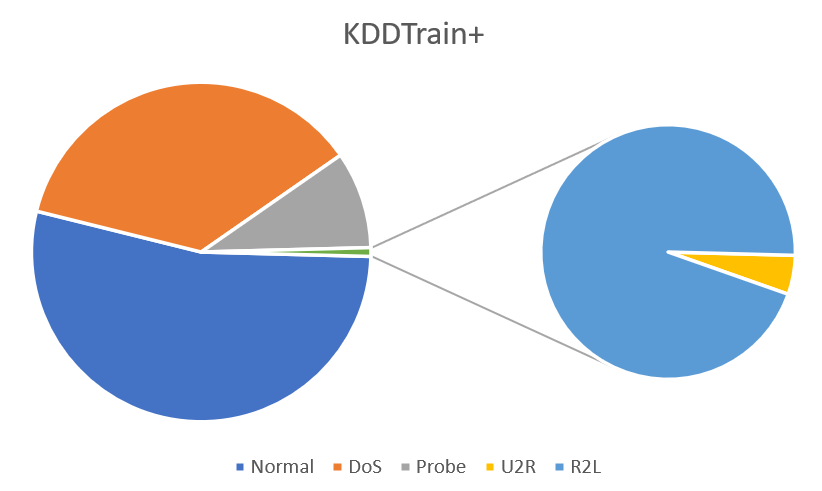
\includegraphics[width = 0.8\textwidth]{kddtraindistribution.png}
    \caption{NSL-KDD完整训练集分类占比饼状图}
    \label{fig:kddtraindistribution}
  \end{figure}

  \begin{figure}[htbp]
    \centering
    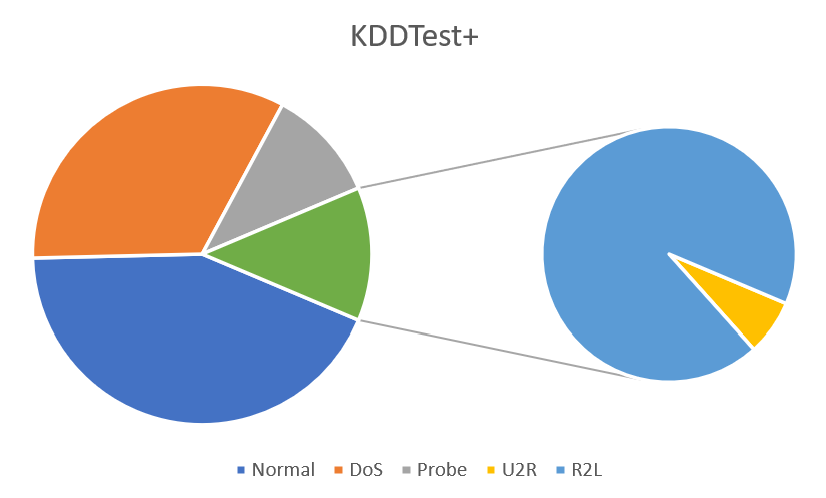
\includegraphics[width = 0.8\textwidth]{kddtestdistribution.png}
    \caption{NSL-KDD完整测试集分类占比饼状图}
    \label{fig:kddtestdistribution}
  \end{figure}


\section{增量学习}

\section{基于遗传算法优化的数据分层抽样}
在数据集预处理过程中,数据抽样操作是一项关键步骤,尤其在处理大规模数据集时。
它不仅能帮助减少计算资源的消耗,还能在一定程度上避免模型过拟合。
数据抽样通常被用来从一个大型数据集中选取一个代表性的子集,以进行更为快速和高效的分析。\par
数据抽样的基本目标是确保选取的样本能够尽可能地反映出总体数据的特性,包括数据的分布、均值、方差等统计属性。
抽样方法大致可以分为两大类:\textbf{概率抽样}和\textbf{非概率抽样}。\par

在概率抽样中,每个样本被选中的概率是已知的,这保证了样本的代表性。
概率抽样的方法包括简单随机抽样、系统抽样、分层抽样和簇抽样等。
在非概率抽样中,样本的选择依赖于研究者的主观判断,而非随机机制,因此每个样本被选中的概率是未知的。
常见的非概率抽样方法包括方便抽样、判断(或目的性)抽样和配额抽样等。\par


\textbf{分层抽样}是一种高效的概率抽样技术,特别适用于处理不均衡数据集。
这种方法的核心优势在于它确保了数据集中所有关键的子群体在样本中都能得到适当的代表性。
在不均衡数据集的情况下,少数类别的样本容易在随机抽样过程中被遗漏,尤其是当这些类别的样本数量极少时。
分层抽样通过保障这些少数类别在样本中的充分代表性,显著提升了模型对这些类别的识别能力。\par

此外,分层抽样通过确保样本中所有相关子群体的均匀分布,有助于降低样本的方差,进而提高估计的准确性。
这一点对于不均衡数据集尤为重要,因为少数类别对模型的整体性能可能产生显著影响。
通过在训练过程中考虑到数据集中的所有子群体,分层抽样促进了模型的泛化能力,使模型能够更有效地处理现实世界数据的多样性与复杂性。
通过图~\ref{fig:kddtraindistribution}、\ref{fig:kddtestdistribution}和\ref{fig:UNSW-NB15barchart}~明显可以看出,本文采用的数据集是非常不均衡的,因此本文将会使用分层抽样对数据集进行处理。
然而对于分层抽样的最佳比率,却不能通过直观的获取到。为了取得最优的抽样比率,本文将会利用遗传算法对分层抽样进行优化。
对于遗传算法,本文已在第~\ref{eq:GA}~章介绍,这里不再赘述,只给出具体实施细节。\par

\textbf{分层抽样}是一种高效的概率抽样技术,特别适用于处理不均衡数据集。
这种方法的核心优势在于它确保了数据集中所有关键的子群体在样本中都能得到适当的代表性。
在不均衡数据集的情况下,少数类别的样本容易在随机抽样过程中被遗漏,尤其是当这些类别的样本数量极少时。
分层抽样通过保障这些少数类别在样本中的充分代表性,显著提升了模型对这些类别的识别能力。\par

此外,分层抽样通过确保样本中所有相关子群体的均匀分布,有助于降低样本的方差,进而提高估计的准确性。
这一点对于不均衡数据集尤为重要,因为少数类别对模型的整体性能可能产生显著影响。
通过在训练过程中考虑到数据集中的所有子群体,分层抽样促进了模型的泛化能力,使模型能够更有效地处理现实世界数据的多样性与复杂性。
通过图~\ref{fig:kddtraindistribution}、\ref{fig:kddtestdistribution}和\ref{fig:UNSW-NB15barchart}~明显可以看出,本文采用的数据集是非常不均衡的,因此本文将会使用分层抽样对数据集进行处理。
然而对于分层抽样的最佳比率,却不能通过直观的获取到。为了取得最优的抽样比率,本文将会利用遗传算法对分层抽样进行优化。
对于遗传算法,本文已在第~\ref{eq:GA}~章介绍,这里不再赘述,只给出具体实施细节。\par

(1) 遗传算法的选择\par
遗传算法的种类以及策略多种多样,在这里我们选择采用稳态遗传算法(Steady State Genetic Algorithm, SSGA)作为优化策略。
与传统的遗传算法相比,稳态遗传算法的特点在于每次迭代只替换种群中的一小部分个体,而不是进行全种群的更新。
这种方法的优势在于绝大多数个体在迭代过程中保持不变,从而避免了每次迭代都进行完整的种群更换。\par

考虑到本文中个体适应度评估的复杂性——每个个体的评估需要经过完整的模型训练及性能评估过程——采用标准遗传算法(即采用完全生成替换策略的遗传算法,其中每次迭代都替换整个种群)将显著增加计算负担,并可能不利于优良基因的保留。
相反,稳态遗传算法通过每次只替换部分种群的策略,不仅大幅度降低了计算量,而且有助于保持种群中的优秀个体。
这种策略的实施有助于加速算法的收敛过程,并且,通过有效地保留高质量的解,稳态遗传算法能够在全局搜索和局部搜索之间取得更好的平衡,从而提高发现全局最优解的可能性。

(2) 特征编码\par
在处理数据集时,特别是在进行增量学习或批量训练时,合理地选择样本是至关重要的。
为了实现这一目标,本文将会利用样本类型的抽样比重来进行特征编码。
遗传算法的每个个体(或称为“染色体”)代表一种可能的样本选择方案,其中包含了对应于数据集中每种样本类型的抽样比重。
这些比重被编码为位于$[0,1)$区间的小数,分别表示各类型样本在总体抽样策略中的比重。
以UNSW-NB15数据集为例,一个可能的染色体编码可以是{0.2, 0.3, 0.1, 0.5, 0.3,0.1,0.2,0.1,0.4,0.1},这分别对应于十种样本类型的采样比重。
需要注意的是,这些比重在实际应用中将会具体调整为抽样百分比。
在进行实际训练时,通过计算训练集样本数量与各类样本抽样百分比的乘积,便可得到每类样本具体的抽样数量。
例如,对于样本数量为100,000的数据集,该染色体对应的每类样本采样百分比、采样数量如表~\ref{tab:Ga_code}~所示。\par

\begin{table}
  \caption{遗传算法编码方案}
  \label{tab:Ga_code}
  \centering
  \begin{tabular}{cccc}
    \toprule
    \textbf{编码值(基因)}&\textbf{样本类型}&\textbf{采样百分比}&\textbf{抽样数量}\\
    \midrule
    0.2&normal&8.695652\%&8696\\
    0.3&Fuzzers&13.043478\%&13043\\
    0.1&Reconnaissance&4.347826\%&4348\\
    0.5&Shellcode&21.73913\%&21739\\
    0.3&Analysis&13.043478\%&13043\\
    0.1&Backdoors&4.347826\%&4348\\
    0.2&DoS&8.695652\%&8696\\
    0.1&Exploits&4.347826\%&4348\\
    0.4&Generic&17.391304\%&17391\\
    0.1&Worms&4.347826\%&4348\\
    \bottomrule
  \end{tabular}
\end{table}

(3) 适应度评估\par
在本文中将会利用染色体基因对应的采样比率对训练集进行SMOTE增强,并利用各个模型在增强后的训练集上进行训练。
最后再在验证集上使用weighted avg-score(公式~\ref{eq:val_score5}~)作为评价标准进行评估,评估值便作为该染色体对应的适应度。
这里没有选用accuracy\_score而选用weighted avg f1-score的原因是
accuracy\_score 虽然简单直观,易于理解但在在类别不平衡的数据集中可能会产生误导。
例如,如果一个类占95\%的样本,模型总是预测这个主要类别,那么准确率可能达到95\%,但这并不意味着模型具有良好的性能。
而weighted avg f1-score 计算精确度(precision)和召回率(recall)的调和平均,对于每个类别分别计算F1分数,并根据每个类别的样本数(support)进行加权平均。
因此weighted avg f1-score能够综合考虑精确度、召回率以及样本类别数量,即使数据集处于不平衡的情况,也能很好地反映模型的性能。\par

(4) 初始群体生成及迭代次数\par
为了确保算法能够充分探索解空间并增加解的多样性,我们特别注重初代种群的广泛性和迭代过程的深入性。
基于此目的,初始种群规模被设定为1,000个个体。
这一较大的初始种群规模有助于覆盖更广泛的解空间,从而提高找到全局最优解的概率。
同时,为了充分优化解并观察算法的收敛行为,设置了10,000次的迭代次数,以便于算法有足够的时间逐步改进解,并最终接近最优解。\par

\begin{table}[htbp]
  \caption{遗传算法实现}
  \label{tab:genetic_algorithm}
  \centering
  \begin{tabularx}{1.0\textwidth}{cl}
  \toprule
  \multicolumn{2}{l}{\textbf{遗传算法}}\\
  \midrule
  \multicolumn{2}{l}{\textbf{输入}: 种群大小 $P$,基因数量 $G$,代数 $N$,变异率 $M$} \\
  \multicolumn{2}{l}{\textbf{输出}: 适应度最高的染色体} \\
  1& 初始化种群 $pop$ \\
  2& \textbf{for} 每一代 \textbf{in} $N$: \\
  3&\quad 选择两个父代 $p1$ 和 $p2$ \\
  4&\quad 生成两个后代 $c1$ 和 $c2$ 通过 $crossover(p1, p2)$ \\
  5&\quad 对 $c1$ 和 $c2$ 进行 $mutate$ 操作 \\
  6&\quad 将 $c1$ 和 $c2$ 加入到 $pop$ 中 \\
  7&\quad 计算种群中每个个体的适应度 \\
  8&\quad 根据适应度计算每个个体的淘汰概率 \\
  9&\quad 淘汰两个适应度最低的个体 \\
  10& \textbf{return} 适应度最高的染色体 \\
  \bottomrule
  \end{tabularx}
\end{table}

(5) 选择、交叉和变异\par
对于选择策略,本文采用轮盘赌选择法,该方法根据个体适应度相对于总体适应度的比例来分配选择概率。
这种方法的优势在于能够有效保证高适应度个体被优先选择,从而引导种群朝着更优解空间方向进化。
在交叉操作方面,为了降低计算的复杂度,本文选择了单点交叉方法。
对于变异策略,本研究设置了0.1的固定概率对新生成的个体中的所有基因进行变异。
在确定变异位置后,以相等的概率选择将该基因值进行1.2倍的放大或0.8倍的缩小。
这样做的目的是保证个体的基因以较小的变化幅度进行细微调整,增强种群的探索能力,同时避免过大的变异导致优秀基因的丢失。
表~\ref{tab:genetic_algorithm}~是我们遗传算法实现的伪代码。




\section{基于ResNet-BiGRU攻击检测模型及IGPPM溯源框架实现}

\section{实验评估与分析}
\subsection{实验环境}
为了评估本文所提方案的有效性,本文将利用python语言来实现以上流程,并选用表~\ref{tab:env_setting}~中的配置来进行实验。
\begin{table}[htbp]
  \caption{实验设备配置}
  \label{tab:env_setting}
  \centering
  \begin{tabular}{ccc}
    \toprule
    \textbf{环境类别} & \textbf{设备项目} & \textbf{项目参数}\\
    \midrule
    \multirow{6}{*}{硬件环境}& CPU型号 & Intel(R) Core(TM) i7-11800H\\
                            & CPU规格 & 8核16线程@2.30GHz\\
                            & GPU型号 & NVIDIA GeForce RTX 3060 Laptop GPU\\
                            & 内存大小& 16.0 GB\\
                            & 硬盘类型& SSD\\
                            & 硬盘大小& 1TB\\
                            \hline
    \multirow{3}{*}{软件环境}&操作系统&Windows 11\\
                            &开发语言&Python 3.11.7\\
                            &编辑器 &Visual Studio Code\\                       
    \bottomrule
  \end{tabular}
\end{table}

\subsection{评估指标}

\subsection{遗传算法优化的分层抽样实验评估}

\subsection{攻击检测及溯源框架实验评估}
